\documentclass[10pt, conference]{IEEEtran}

\usepackage{subimages}
\usepackage[cmex10]{amsmath}
\interdisplaylinepenalty=2500
\usepackage{amsthm}
\newtheorem{definition}{Definition}

\usepackage[draft]{hyperref}
\usepackage{todonotes}
\usepackage{float}
\usepackage[english, brazil]{babel}
\usepackage[utf8]{inputenc}
\usepackage[T1]{fontenc}
\usepackage{url}
\usepackage{minted}
\usepackage{subfig}
\usepackage{verbatim}
%\usepackage{geometry}% http://ctan.org/pkg/geometry
%\usepackage{lipsum}% http://ctan.org/pkg/lipsum
%\usepackage{graphicx}% http://ctan.org/pkg/graphicx
\hyphenation{op-tical net-works semi-conduc-tor}


\begin{document}

\title{Problema de Detecção Facial utilizando RCNN}

\newif\iffinal
%\finalfalse
\finaltrue
\newcommand{\jemsid}{99999}


\iffinal
  \author{%
    \IEEEauthorblockN{Rodolfo Labiapari Mansur Guimarães}
    \IEEEauthorblockA{%
    Departamento de Computação\\
    Universidade Federal de Ouro Preto - UFOP\\
    Ouro Preto - MG -- Brasil\\
    \href{mailto:rodolfolabiapari@decom.ufop.br}{rodolfolabiapari@decom.ufop.br}}
  }
\else
  \author{Sibgrapi paper ID: \jemsid \\ }
\fi

\maketitle



\selectlanguage{english}
\begin{abstract}
	In this article, a face detector implementation is presented using a neural network architecture using the \textit{neon} tool, developed to detect robustly face patterns. The use of neural network to detect objects is necessary because of the high difficulty of computational models to be successful in detecting objects in images where there are complex environments and variations of the object as the faces. The implemented system automatically synthesizes the problem-specific for extracting features from a standard set of faces and nonfaces, without any human interference to extract and create patterns. The procedure works as a pipeline convolutions and subsampling, eliminating data that is not relevant for processing. Techniques that use convolutional neural network type architecture are emphasizing in the academic environment, because it is a procedure that obtains results with good accuracy and without having great losses with the respective trade-off and can even be used for classifications in low-power processing environments such as personal computers and even embedded systems.

	\begin{IEEEkeywords}
		Face Detection; Convolutional Neural Network; API \textit{neon} Intel Nervana.
	\end{IEEEkeywords}
\end{abstract}


\selectlanguage{brazil}
\begin{abstract}
	Neste artigo, é apresentado uma implementação de detector de face utilizando uma arquitetura de rede neural convolucional por meio da ferramenta \textit{neon}, desenvolvido para detectar padrões de faces de forma robusta. O uso de rede neural para detecção de objetos é necessário pela grande dificuldade de modelos computacionais terem sucesso na detecção de objetos em imagens onde existam ambientes complexos e variações do objeto como as faces. O sistema implementado sintetiza automaticamente o problema específico para extração de características de um conjunto padrão de faces e não-faces, sem qualquer interferência humana para extrair e criar padrões. O procedimento funciona como um \textit{pipeline} convoluções e sub-amostragens eliminando dados que não são relevantes para processamento. Técnicas que utilizam arquitetura tipo \textit{convolutional neural network} estão destacando no ambiente acadêmico, por ser um procedimento que obtêm resultados com boa acurácia e sem ter grandes perdas com o respectivo \textit{trade-off} podendo até ser usado para classificações em ambientes de baixo poder de processamento como computadores pessoais e até sistemas embarcados.
	
	\begin{IEEEkeywords}
		Detecção de Face; Rede Neural Convolucional; API \textit{neon} Intel Nervana.
	\end{IEEEkeywords}
\end{abstract}



\IEEEpeerreviewmaketitle


\section{Introdução}
	Detecção de face é um problema pertencente à visão computacional no qual, métodos têm como propósito a detecção de faces.

	Esse problema se torna difícil quando não se tem imagens com ambientes controlados tal como um fundo controlado, ou seja, com um \textit{background} que não respeite um padrão pré-estabelecido, com obstrução facial como óculos, barba, etc \cite{Garcia2004}.

	Como o estado da arte é concreto em detecção de face em ambientes controlados, pesquisas nas últimas décadas partem a buscar métodos que focam principalmente na detecção de face em ambientes onde existe maior complexidade, sem perder a eficiência já conseguida até então. As pesquisas em detecção de face hoje procuram métodos eficientes e rápidos onde as faces podem se apresentar não só posicionada em perfil mas sim, com distâncias, angulações e rotações variadas, oclusões,níveis extremos de iluminação, entre outras variações que poderiam representar situações que representassem o mundo real na captura de imagens comuns \cite{Haoxiang2015}.

	\textit{Deep convolutional neural network} também conhecida como \textit{convolutional neural network} (CNN) é uma arquitetura de rede neural que foi introduzida com grande sucesso por Le Cun et al \cite{LeCun1989} \cite{LeCun1990H} \cite{LeCun1998G} que é baseada em rede neural, apresentada por McCulloch \cite{McCulloch1943}. São bioinspirados em rede neural multicamada hierárquica que combinam três técnicas arquitetônicas para assegurar graus de invariância de mudança, escala e distorção com procedimentos de campos receptivos locais, pesos compartilhados e sub-amostragem (\textit{subsampling}) espacial. Com isso, diferentes arquiteturas baseadas na rede neural convolucional tem sido utilizadas com sucesso pela literatura em inúmeras aplicações com grau de dificuldade elevada como reconhecimento de escrita à mão  \cite{LeCun1990H}, reconhecimento de caracteres de máquinas de escrever \cite{Martin1991} \cite{Wang1993} e reconhecimento de faces \cite{Lawrence1997}.

	Vaillant et al. \cite{Vaillant1994} usou uma rede convolucional para detecção de objetos baseado em imagens e considerou o caso como um problema o de detecção de face. Garcia et al. \cite{Garcia2004}, em seu trabalho, propõe uma abordagem diferente de reconhecimento de faces alterando as disposições e configurações das camadas da rede neural. Nomeiam seu algoritmo como \textit{Convolutional Face Finder} no qual consiste de num algoritmo de rede neural composto por um \textit{pipeline} de camadas convolucionais. O algoritmo apresentado por eles possui seis camadas, com exceção da camada de recebimento da imagem de entrada. As quatro primeiras camadas são um grupo chamado de mapa de características onde é realizado uma convolução e \textit{subsampling} na imagem, no qual é repetido por duas vezes. Após o mapas de características, há uma camada de rede neural totalmente conectada com o propósito de definir de fato o resultado dos cálculos feitos pelas redes convolucionais, que no caso é um problema de decisão.

	O trabalho conta também com o uso de uma API para a confecção do trabalho onde utilizou-se da API \textit{neon} da Intel Nervana.

	O artigo está disposto da seguinte forma: Seção \ref{sec:justificativa} define justificativas para a realização deste trabalho e um referencial teórico abordando o funcionamento da ferramenta para cumprir seu propósito na Seção \ref{sec:rt}. Na Seção \ref{sec:desenvolvimento} é descrito em detalhes o processo de reconhecimento de face utilizando arquitetura \textit{convolutional neural network} enquanto na Seção \ref{sec:experimentos} é feita as considerações e na Seção \ref{sec:resultados} é descrito os resultados obtidos. Na Seção \ref{sec:conclusao} é feito conclusões e propostas para futuras pesquisas.

\section{Justificativa} \label{sec:justificativa}
	Sistemas computacionais anteriores à redes neurais possuíam características bastante ineficientes para imagens que tinham como propriedade fundos não-padronizados \cite{Garcia2004}.

	Considerando o sucesso de algoritmos que utilizam \textit{convolutional neural network} em reconhecimento de padrão em tarefas, como será descrito na Seção \ref{sec:rt}, a literatura afirma que é possível ter bons resultados utilizando tal API para reconhecer faces faces, em imagens não padronizadas. E como a API não é \textit{ad-hoc}, é possível utilizá-la em vários outros conjuntos de problemas criando assim um algoritmo robusto para detecção de padrões \cite{Haoxiang2015}.

\section{Referencial Teórico} \label{sec:rt}
	\subsection{\textit{Convolutional Neural Network}}
		O algoritmo baseia-se em vários pequenos processos. São eles a \textit{Convolution}, \textit{Subsampling} e a mescla dos dois processos formando o maior chamado de mapa de características e por fim uma rede totalmente conectada para gerar a decisão final \cite{Garcia2004}.

		O primeiro passo do mapa de características é a extração dessas. A primeira camada realiza uma convolução de um filtro gerado pelo algoritmo sobre a imagem a fim de encontrar características específicas da imagem. Com o resultado da convolução, para dar continuidade ao algoritmo e iniciar o próximo procedimento deve-se realizar o processo de filtro onde a saída do primeiro passa por avaliações antes de dar entrada no segundo. Nesse filtro, realiza-se o processo de \textit{Subsampling} no qual utiliza o algoritmo de \textit{max\_pooling} para reduzir o tamanho de amostras a ser processada. Esses dois processos descritos formam o mapa de características. A finalidade deste mapa trata-se da prática de aplicar repetidas vezes a saída do grupo como entrada do próximo e quantas vezes forem estabelecidas. Assim, o resultado de uma convolução, após o \textit{subsampling}, resulta na entrada do próximo processo a ser realizado \cite{Garcia2004} \cite{Giusti2013}. 

		\subsubsection{Alimentação e Funcionamento}
			Diferente das redes neurais totalmente conectadas, oo invés de usar uma imagem inteira como alimento para a rede neural, utiliza técnicas mais elaboradas para extrair uma vantagem maior.

			O processo de convolução é realizado sobre imagens de pequeno porte, contornando o gasto de energia processando uma imagem inteira. Dessa forma, é selecionado uma imagem de no mínimo $ 20 \times 20 $ e os processos de convolução, \textit{pooling} e decisão são feitas somente nesta pequena imagem. Com isso, não possui o gasto desnecessário de energia e tempo processando uma imagem completa. Para este procedimento ser aplicado em qualquer imagem, realiza o processo de seleção de regiões para as classificações. Este processo é realizado primeiramente quebrando a imagem em vários quadros\footnote{Semelhante a ideia de Janelas Deslizantes.} e realiza o processo do mapa de característica em cada uma das pequenas imagens. Os resultados dos \textit{pooling} serão salvos numa matriz que segue a indexação da imagem original. Ela é gerada com a avaliação da convolução gerada em conjunto com o algoritmo de \texttt{max\_pooling} onde selecionará o melhor resultado em determinado quadrante resultando em uma matriz só de soluções com valores avaliados como melhores. Este processo chama-se \textit{Redução de Amostragem}  \cite{Garcia2004} \cite{Giusti2013}.

			A função \texttt{max\_pooling} é uma forma de sub-amostragem não-linear. Ela particiona a imagem de entrada em um conjunto não sobreposto de retângulos e para cada tipo de sub-região, retorna o máximo valor encontrado. Seu propósito é a eliminação de valores não maximais reduzindo o processamento computacional nas camadas posteriores. Ela também provê uma forma de transação invariante no processo realizado. Isso provê uma robustez adicional na posição, ela também é uma forma inteligente de reduzir a dimensionalidade de representações intermediárias do processo. O processo é demonstrado na Figura \ref{fig:max_pooling.png}.

			\begin{figure}[h]
				\centering
				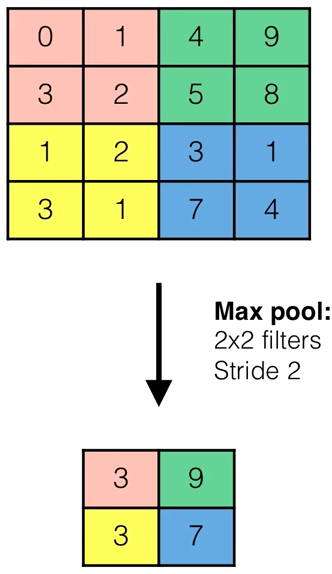
\includegraphics[width=0.4\linewidth]{img/max_pooling.png}
				\caption{O processo de seleção de melhores resultados. Procedimento executado pela função \texttt{max\_pooling}.}
				\label{fig:max_pooling.png}
			\end{figure}

			Feito todos os passos do mapa de características, utiliza-se cada quadro gerado pela última redução em uma pequena rede neural para a geração da decisão final.
			
			Com esses processos que são anteriores a pequena rede neural, elimina-se os itens irrelevantes para o processamento sem perder a acurácia do algoritmo. 

			Os itens resultantes serão entrada para outra rede neural que fará de fato a decisão final. Esse último explora a correlação espacial reforçando um padrão de conectividade local entre neurônios nas camadas adjacentes, ou seja, as entradas da camada $ m $ são de um conjunto da camada anterior $ m-1 $ relacionados de uma forma contígua como é exibido na Figura \ref{fig:layers_cnn} \cite{LeCun1989} \cite{LeCun1990H}.
			
			\begin{figure}[h]
				\centering
				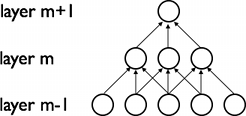
\includegraphics[width=0.8\linewidth]{img/layers_cnn.png}
				\caption{Exemplo das camadas de uma rede \textit{convolutional neural network}.}
				\label{fig:layers_cnn}
			\end{figure}
			
			
			Tal teoria é exibida na Figura \ref{fig:convolucao_teoria}. Posta uma imagem de qualquer tamanho como entrada, ela será dividida em vários blocos cujo tamanho é referente à especificado pelo algoritmo de convolução. Serão realizado os métodos de convolução em cada bloco e estes serão salvos numa matriz. Um procedimento de otimização avaliará a matriz a fim de eliminar todos os dados que forem irrelevante para o problema, sendo esses dois processos podendo repetir caso pré-definido. Com a matriz de resultados promissores em mão, é executado um algoritmo de rede neural para avaliar quais blocos são de suas respectivas classes, de acordo com o treino realizado.

			\begin{figure*}[h]
				\centering
				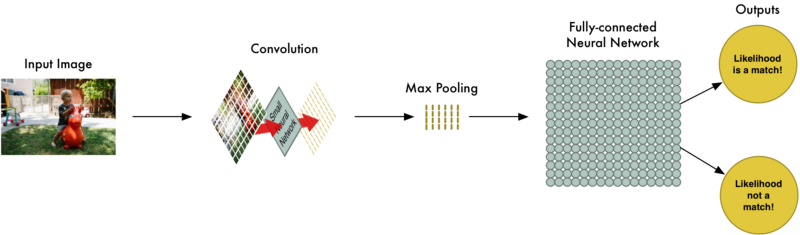
\includegraphics[width=1.0\linewidth]{img/convolucao_teoria.png}
				\caption{O processo simples de uma arquitetura de reconhecimento de padrão \textit{convolutional neural network} final após todos os processos.}
				\label{fig:convolucao_teoria}
			\end{figure*}

			Com tais procedimentos, conclui-se o processo de avaliação utilizando \textit{convolutional neural network}. Um exemplo geral é exibido na Figura \ref{fig:cnn_geral} no qual, cada pedaço da imagem $ R $ é recortado e selecionado, feito os processos de convolução por meio dos mapas de características $ \varphi_n $ e em seguida a pela rede neural totalmente conectada $ \Omega $ que produz a decisão final $ \varPsi $.
			
			\begin{figure}[b]
				\centering
				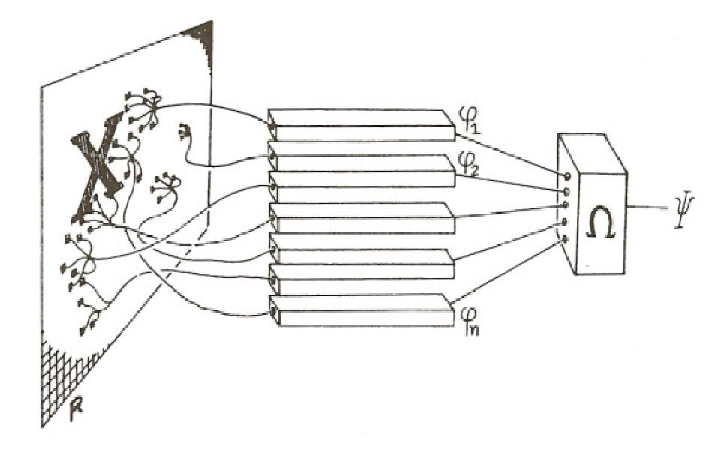
\includegraphics[width=0.9\linewidth]{img/single_layer_cnn.png}
				\caption{Exemplo de identificação de rosto especificado pelo \textit{data set} disponibilizado pela Universidade de Massachusets Amherst.}
				\label{fig:cnn_geral}
			\end{figure}


	\subsection{\textit{neon}} \label{sec:neon}
		Segundo a sua documentação, \textit{neon} é uma \textit{API} de código-aberto, um projeto de \textit{deep learning} referente ao Intel Nervana desenvolvido para ter excelente performance em qualquer \textit{hardware} além de ser planejado para ser fácil de uso e extensível à outros recursos \cite{neon}.

		Entre suas várias características, as principais são:

		\begin{itemize}
			\item Suporte aos modelos mais comuns utilizados hoje como \textit{convnets}, RNN, LSTM e outros;
			\item Modelos pré-treinados, pronto para uso;
			\item Integração com o bibliotecas Kernel de GPUs;
			\item Suporte a diferenciação automática básica;
			\item \textit{Backends} de \textit{hardware} adaptável, ou seja, é possível escrever o código em um local e portar para CPU, GPU, ou \textit{hardware} próprio da Nervana.
		\end{itemize}

		Para seu treinamento e classificação, o algoritmo necessita especificamente de um \textit{data set}, uma lista de camadas que fará a composição da arquitetura da rede, uma função de custo e uma regra de aprendizagem que no qual gerará a rede neural requerida para detecção.

		A API disponibilizada é desenvolvida em linguagem de programação Python. Como é uma API de distribuição gratuita e executada em modo local, necessita de instalação de suas bibliotecas \textit{kernel} na máquina a ser realizada os treinos e teste. Assim, para realizar a instalação, basta utilizar os seguintes comandos:

		\begin{minted}[
		numberblanklines=true,
		numbersep=12pt,
		numbersep=12pt,
		gobble=0,
		frame=lines,
		framerule=0.4pt,
		framesep=2mm,
		tabsize=4,
		obeytabs=true,
		samepage=false, %with this setting you can force the list to appear on the same page
		showspaces=false,
		showtabs =false,
		linenos
		]{shell}
git clone \
https://github.com/NervanaSystems/neon.git
cd neon && make sysinstall
		\end{minted}

		O processo de construção da rede neural passa por cinco itens principais. O primeiro é a geração de um \textit{backend}, no qual realiza o procedimento de inicialização e definição de onde o algoritmo será executado (CPU, GPU, ...). O segundo é o carregamento do \textit{data set}, podendo ser alguns já disponíveis pelo próprio projeto ou mesmo realizando o carregamento de um específico para treino e avaliação. O na parte de treino terceiro, deve-ser realizar a especificação do modelo de arquitetura da rede onde se define itens como as camadas, funções de ativação e os pesos dos iniciadores. Após o treinamento, é possível realizar a avaliação da rede.


\section{Desenvolvimento} \label{sec:desenvolvimento}

	\subsection{Uso dos Data set}
		Para o treino e avaliação, utilizou-se de dois conjuntos de dados e \textit{benchmark} disponibilizado gratuitamente.

		Todos os data sets foram encontrados por meio do sítio \url{http://www.face-rec.org/databases/} no qual fornece informações básicas das mais variadas bases para estudo e aplicação em pesquisa.

		\subsubsection{\textit{faces94}} \label{sec:94}
			Para geração de faces, utilizou-se de um conjunto de dados disponível pela Universidade de Essex, na \textit{School of Computer Science and Electronic Engineering}, Inglaterra, disponível em \url{http://cswww.essex.ac.uk/mv/allfaces/faces94.html}.

			No conjunto utilizado, os indivíduos foram fotografados numa distância fixa da câmera e solicitados para que falem enquanto as fotos foram tiradas. O processo de fala produz expressões faciais nos indivíduos, criando maior variabilidade no conjunto de dados a ser utilizado para treino.

			Todas as imagens coloridas possuem plano de fundo verde, as cabeças possuem variações naturais de rotação, movimento e posição, não possui variação de luminosidade, possui um numero considerável de expressões mas nenhuma com alto nível.

			O \textit{data set} possui um total de 153 indivíduos, com imagens de resolução fixa no valor de $ 180 \times 200 $ e com três sub-diretórios nomeados: \textit{male}, \textit{female} e \textit{malestaff} e a quantidade de seus respectivos indivíduos: 20, 113 e 20.


		\subsubsection{FDDB: Face Detection Data Set and Benchmark} \label{sec:FDDB}
			Disponibilizado pela Universidade de Massachusets Amherst \cite{fddbTech}, o \textit{data set} possui um conjunto de anotações para 5171 faces identificadas num conjunto de 2845 imagens retiras do conjunto nomeado \textit{Faces in the Wild}, disponível em \url{http://tamaraberg.com/faceDataset/index.html}. O conjunto inteiro possui um total de 30281 imagens com faces coletadas da fonte \textit{News Photographs}. Todas foram automaticamente etiquetadas por meio do sistema descritivo \textit{Who's in the Picture}, no qual possui 80\% de acurácia \cite{berg2004s}.

			Os dados estão em formato compactado \texttt{jpg}. Junto com o pacote de imagens, existe um arquivo com o seguinte formato:

			\begin{verbatim}
				...
				<image name i>
				<number of faces in this image =im>
				<face i1>
				<face i2>
				...
				<face im>
				...
			\end{verbatim}

			onde cada face é denotada por

			\begin{verbatim}
				<major_axis_radius minor_axis_radius angle
				 center_x center_y 1>
			\end{verbatim}

			no qual tais valores representam a posição da face como é exibido na Figura \ref{fig:mulher}.

			\begin{figure}[h]
				\centering
				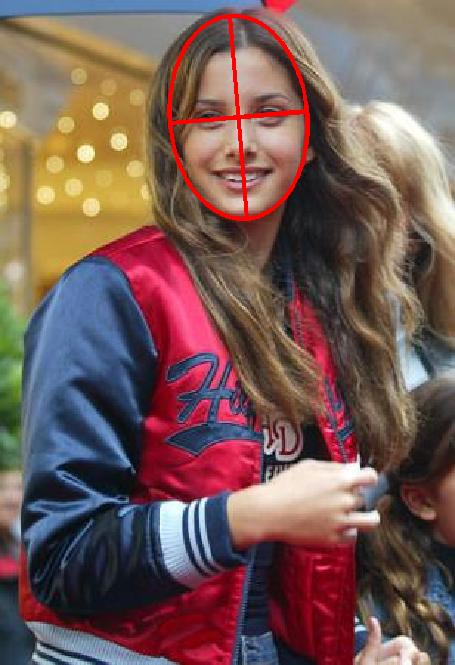
\includegraphics[width=0.8\linewidth]{img/data_set.jpg}
				\caption{Exemplo de identificação de rosto especificado pelo \textit{data set} disponibilizado pela Universidade de Massachusets Amherst.}
				\label{fig:mulher}
			\end{figure}
		
			Possui ao total dez sub-diretórios separados aleatoriamente, todos com informações de localização de face. Tais diretórios possuem quantidades de imagens diferentes, mas todos possuem uma média de 280 imagens.
			
		\subsubsection{Disposição para Uso}
			\paragraph{Conjunto \texttt{faces\_set}}
				Como as imagens do \textit{faces94} só possui a face dos indivíduos, tais como são os porta-retratos, esse conjunto de dados foi exclusivamente utilizado para treinar a rede sobre as características de faces. As imagens são modificadas para escala de cinza (Figura \ref{fig:94_colored}) e recortadas para terem o formato quadrado (Figura \ref{fig:94_cut}), padrão de entrada do algoritmo.

				\begin{figure}[h]
					\centering
					\subfloat[Face 1]{{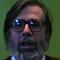
\includegraphics[width=0.25\linewidth]{img/94_colored.jpg} }}%
					\qquad
					\subfloat[Face 2]{{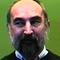
\includegraphics[width=0.25\linewidth]{img/94_colored_2.jpg} }}%
					\caption{Faces do \textit{data set Faces94}. Imagens colorias, com tamanho $ 180 \times 200 $ e com expressões faciais}%
					\label{fig:94_colored}%
				\end{figure}
				
				\begin{figure}[h]
					\centering
					\subfloat[Face 1 Cortada]{{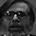
\includegraphics[width=0.25\linewidth]{img/94_cut.jpg} }}%
					\qquad
					\subfloat[Face 2 Cortada]{{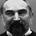
\includegraphics[width=0.25\linewidth]{img/94_cut_2.jpg} }}%
					\caption{As respectivas faces já processadas e prontas para treino.}%
					\label{fig:94_cut}%
				\end{figure}
			
				Utilizando todas as imagens \texttt{.jpg} deste conjunto, tem-se o total de 2980 faces prontas para treino.

				O conjunto \textit{FDDB} poderia ser utilizado para a geração de novas imagens de grupo \texttt{face} complementando o grupo já formado pelo \textit{faces94} já que é grande o suficiente para o recorte das faces já que tem-se a localização de cada uma. Entretanto, mesmo com suas indicações de faces em documento texto, não foi viável utilizá-las para treino pelo motivo de que algumas unidades de faces estão incompletas por causa de obstruções ou por estarem não totalmente exibidas por completo. Faces com desfoque, com pedaços obstruídos por óculos, barbas, distorções da imagem ou mesmo incompleta por algum objeto.
				
				Tentar utilizá-lo eliminando as faces obstruídas entraríamos novamente no problema de detecção já que seria inviável fazer o processo manualmente pelo motivo do conjunto conter inúmeras imagens podendo ter até várias unidades de rostos cada uma.
				
				Dessa forma, o conjunto \textit{FDDB} foi desconsiderado totalmente para a geração de faces para treino.
				

			\paragraph{Conjunto \texttt{non\_faces\_set}}
				Para a geração de imagens não-faces, utilizou-se da técnica de selecionar pedaços aleatórios de imagens e etiquetá-las como não-face.

				Como o conjunto \textit{faces94} não possui ambiente suficiente para a geração de imagens não-faces, utilizou-se das imagens do conjunto \textit{FDDB} para a sua geração. Por mais que ele não fosse suficiente para a geração de faces, para não-faces, seu conjunto possui grande utilidade para o corte de inúmeras não-faces para treino.

				Para evitar a geração de imagens que contenham faces o parte delas, utilizou-se das coordenadas conhecidas para evitar áreas que contenham partes de faces. Esse procedimento foi necessário para que os conjuntos de dados não confunda o treino da rede mostrando, por exemplo, uma parte de uma boca e dizer que aquilo não faz parte de uma face, sendo que essa afirmação é falsa.
				
				Com exceção desta restrição, todas as imagens não-faces são geradas de forma aleatória como é exibido na Figura \ref{fig:fddb_cut}.

				\begin{figure}[H]
					\centering
					\subfloat[Não-face 1]{{
\includegraphics[width=0.25\linewidth]{img/fddb_cut.jpg} }}%
					\qquad
					\subfloat[Não-face 2]{{
\includegraphics[width=0.25\linewidth]{img/fddb_cut_2.jpg} }}%
					\qquad
					\subfloat[Não-face 3]{{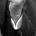
\includegraphics[width=0.25\linewidth]{img/fddb_cut_3.jpg} }}%
					\caption{Algumas imagens recortadas para treino de não-faces.}%
					\label{fig:fddb_cut}%
				\end{figure}
			
			

		\subsubsection{Treino, Teste e Validação}
			Tendo definido as restrições de como será composto cada \textit{data set}, deve-se então separar os grupos de treino, teste e validação.
			
			Para o conjunto \textit{faces94}, todas as imagens foram utilizadas para treino de reconhecimento faces.
			
			O conjunto \textit{FDDB} possui dez subconjuntos nomeados de 1 à 10, todos com descrição de localização de faces. Para a divisão de treino, teste e validação, separou os os conjuntos em três grupos onde os subconjuntos 1 à 4 irá pertencer à imagens utilizadas para recorte de não-faces para treinos, os subconjuntos de 5 à 8 serão utilizados para testes e refinamento dos resultados e os para avaliação e geração de resultados, será utilizado os subconjuntos 9 e 10.

	\subsection{API \textit{neon}}
		Para o uso do \textit{neon}, deve-ser realizar configurações sistêmicas no algoritmo antes de sua execução. As configurações realizadas foram:

			\begin{itemize}
				\item \textbf{\textit{Backends}:} NervanaCPU;
				\item \textbf{\textit{Data sets}:} \textit{face94} e FDDB;
				\item \textbf{\textit{Initializers}:} Uniforme;
				\item \textbf{\textit{Optimizers}:} \textit{Gradient Descent} com Momento;
				\item \textbf{\textit{Activations}:} Linear Retificada, Softmax;
				\item \textbf{\textit{Layers}:} Convolução, Pooling; e
				\item \textbf{\textit{Cost}:} \textit{Multi Cross Entropy}.
			\end{itemize}
		
		Para a arquitetura da rede, precisamente a descrição das suas camadas, utilizou-se de duas camadas de convolução, de \textit{pooling} e de \textit{Affine} que é uma rede neural totalmente conectada. A arquitetura da rede e suas configurações são exibidas a seguir:

		\begin{minted}[
		numberblanklines=true,
		numbersep=12pt,
		gobble=0,
		frame=lines,
		framerule=0.4pt,
		framesep=2mm,
		tabsize=4,
		obeytabs=true,
		samepage=false, %with this setting you can force the list to appear on the same page
		showspaces=false,
		showtabs =false,
		linenos
		]{python}
layers = [
	Convolution(
		fshape=(5, 5, 4), 
		init=init_uni),
	Pooling(fshape=(2, 2)),
	Convolution(
		fshape=(3, 3, 14), 
		init=init_uni),
	Pooling(fshape=(2, 2)),
	Affine(nout=14, 
		init=init_uni, 
		activation=Rectlin(), 
		batch_norm=True),
	Affine(nout=2, 
		init=init_uni, 
		activation=Softmax())   ]
		\end{minted}

		As configurações utilizadas para a realização dos testes foram:

		\begin{itemize}
			\item \textbf{\textit{Batch size}:} 512;
			\item \textbf{\textit{Numbers of epoch}:} 1250;
			\item \textbf{\textit{Size of image} (altura e largura):} 36;
			\item \textbf{\textit{Learning Rate}:} 0.01;
			\item \textbf{\textit{Momentum}:} 0.9;
			\item \textbf{\textit{Type of datas}:} inteiro não sinalizado de 8-bits.
		\end{itemize}

\section{Experimentos} \label{sec:experimentos}
	Para a realização dos experimentos, foi necessário adaptar o algoritmo para o reconhecimento de regiões, também chamado de \textit{Region-based Convolutional Neural Network} (RCNN). Tais algoritmos necessitam que, dada uma imagem de entrada, seja gerado várias regiões da foto que são compatíveis com o tamanho de entrada do algoritmo. 

	Isso é necessário pois a rede neural deve operar sobre toda a imagem, de vários tamanhos possível pois as faces pode estar dispostas de vários tamanhos e posições diferentes na imagem. Entretanto, a entrada do algoritmo requisita uma imagem fixa em formato quadrado para processamento. Para que este requisito possa ser satisfeito, foi feito um processamento de geração de regiões que pega a imagem original a ser avaliada, recorta-a em várias regiões de vários tamanhos diferentes e redimensiona-as para o formato padrão de entrada da rede neural a fim de tentar localizar todas as faces na imagem, independente de sua posição ou tamanho.

	Após a definição de regiões, executa-se o algoritmo em cada uma das regiões. Cada região que for definida, ao final do algoritmo, como uma face, será destacada sobre a imagem original em escala de cinza, como mostra a Figura \ref{fig:detect_} e as Figuras \ref{fig:detect_2}, \ref{fig:detect_3}, \ref{fig:detect_4} e \ref{fig:detect_5} em anexo.

	\begin{figure}[ht]
		\centering
		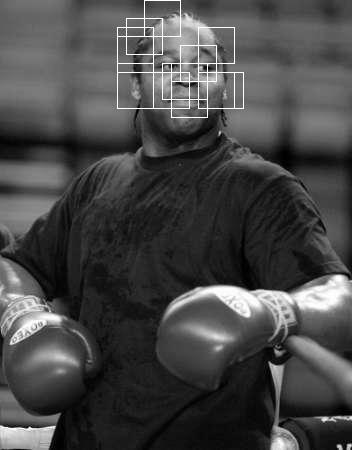
\includegraphics[width=0.75\linewidth]{img/detect.jpg}
		\caption{Exemplo de saída de uma foto após o processo de detecção.}
		\label{fig:detect_}
	\end{figure}


\section{Resultados} \label{sec:resultados}
	Para obtenção de resultados factíveis, as saídas de cada região foram comparadas com os dados fornecidos pelos descritores dos \textit{data sets} de validação. Calculando acertos e distância, é possível encontrar a taxa de acerto do algoritmo e também possíveis melhorias para trabalhos futuros.
	
	A Tabela \ref{tab:erros} exibe o total e percentual de acertos e erros de cada tipo de decisão, processado o número de 929.977 regiões.
	
	\begin{table}[H]
		\centering
		\caption{Valores totais e percentuais de cada tipo de erro dos \textit{data sets} de validação.}
		\label{tab:erros}
		\begin{tabular}{|l|c|c||c|c|}
			\hline
			& \textbf{Numbers} & \textbf{\%}     & \textbf{Numbers} & \textbf{\%}     \\ \hline
			\textit{True Positives}  & 2995    & 55,391 & 2801    & 51,038 \\ \hline
			\textit{False Positives} & 2412    & 44,608 & 2687    & 48,961 \\ \hline \hline
			\textit{True Negatives}  & 239.142 & 49,694 & 239.347 & 54,662 \\ \hline
			\textit{False Negatives} & 242.078 & 50,305 & 198.515 & 45,337 \\ \hline \hline \hline
			\textbf{Total Regions}   & \textit{486.627} & \textit{100}    & \textit{443.350} & \textit{100}    \\ \hline
		\end{tabular}
	\end{table}

	É possível ver que o algoritmo teve um pouco mais de cerca de $ 50\% $ de acerto em suas decisões em todos os \textit{benchmark} testados. Como uma segunda métrica para visualização de sucesso, foi feito uma comparação de todas as regiões testadas com os respectivos pontos centrais de cada face, analisando a distância absoluta entre cada ponto reconhecido e o ponto da face. Na Figura \ref{fig:bp-9}, é possível perceber que os valores de Verdadeiro Positivo possuem, em média, uma distância menor que cem pixels enquanto os Falsos Positivos, por sua vez, possuem uma distância maior do ponto, o que é justificado já que não pertencem à área da face. Os pontos de Falso Positivo são pontos que estão próximo da face, mas que o algoritmo não soube decidir com tanta certeza se foram de fato regiões que pertencem a face ou não. O mesmo padrão pode ser visualizado na Figura \ref{fig:bp-10}.
	
	\begin{figure}[h]
		\centering
		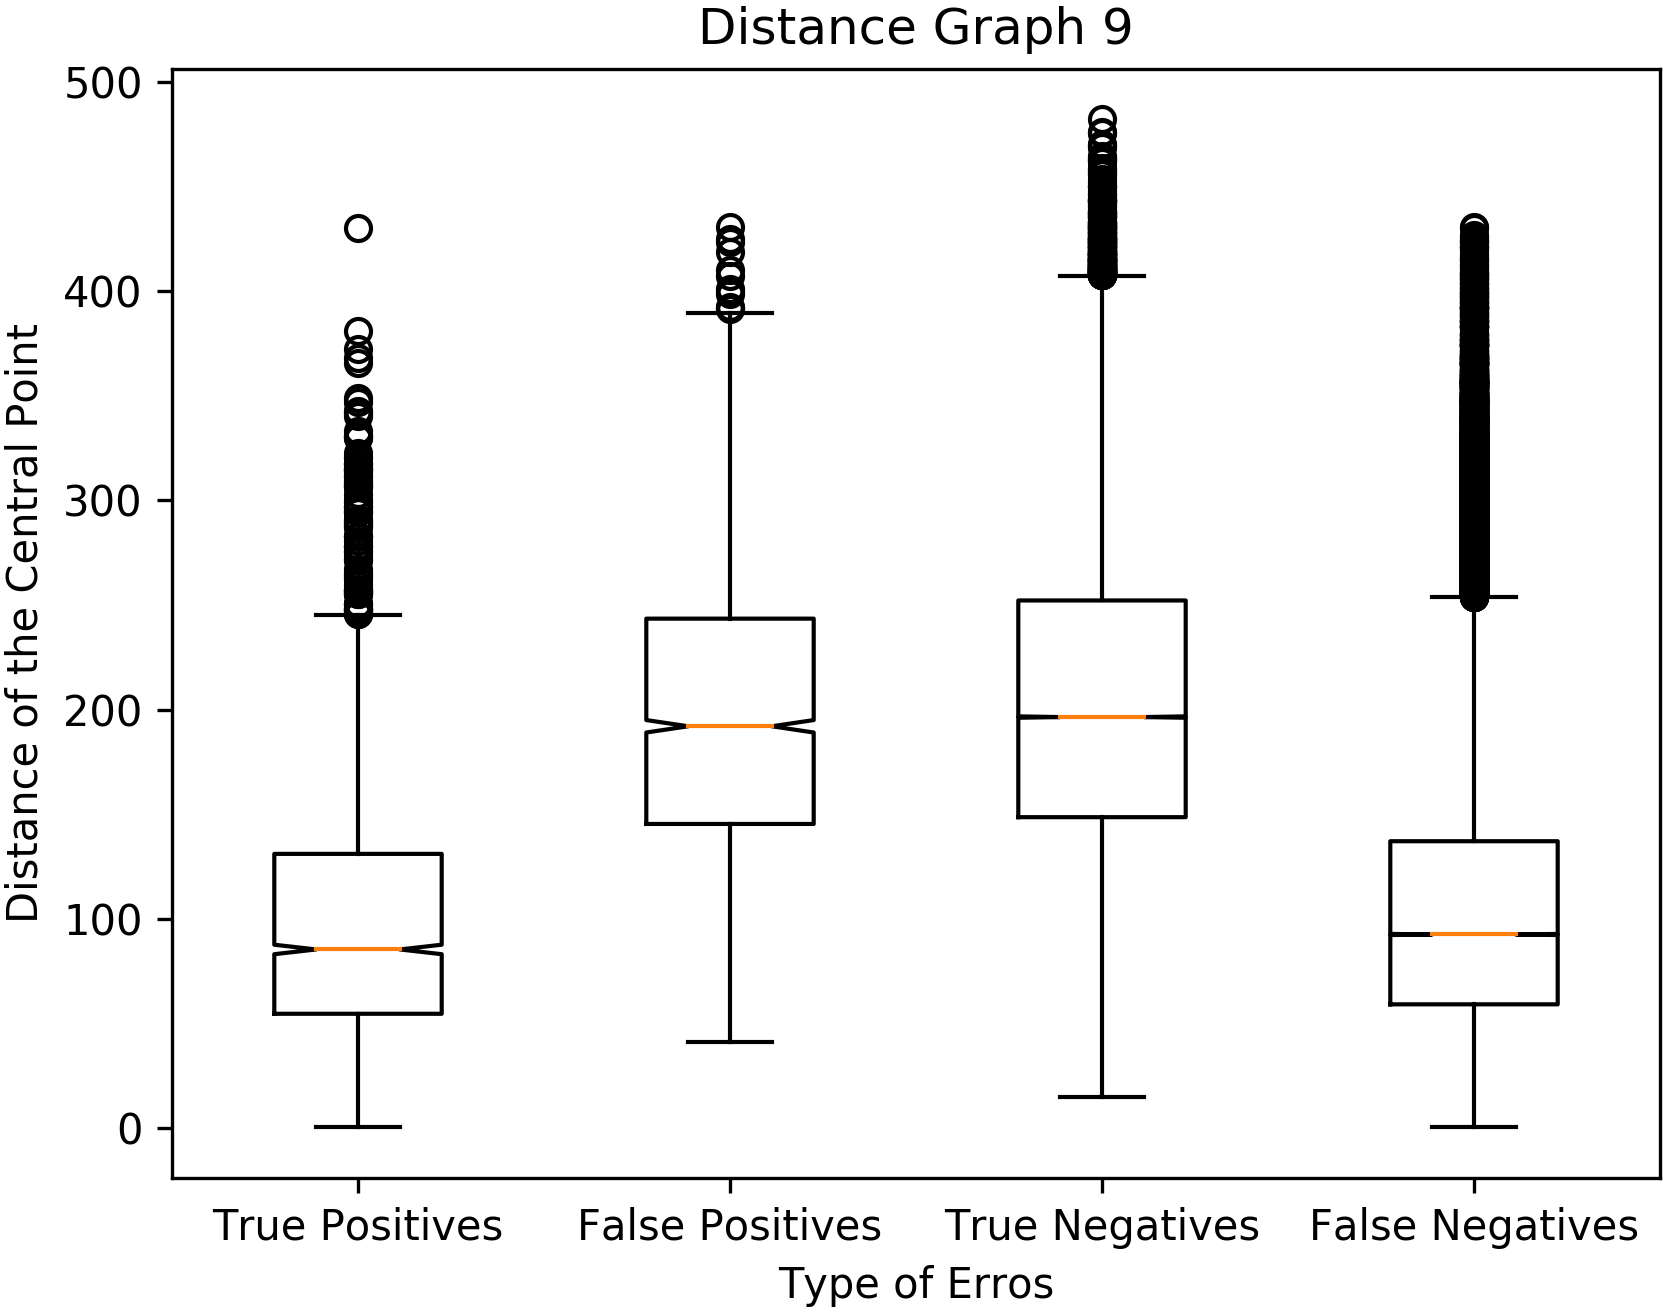
\includegraphics[width=1\linewidth]{img/boxplot-9.png}
		\caption{Exibição das distâncias e valores de erro do \textit{data set} 09 em cada tipo de região.}
		\label{fig:bp-9}
	\end{figure}

	\begin{figure}[h]
		\centering
		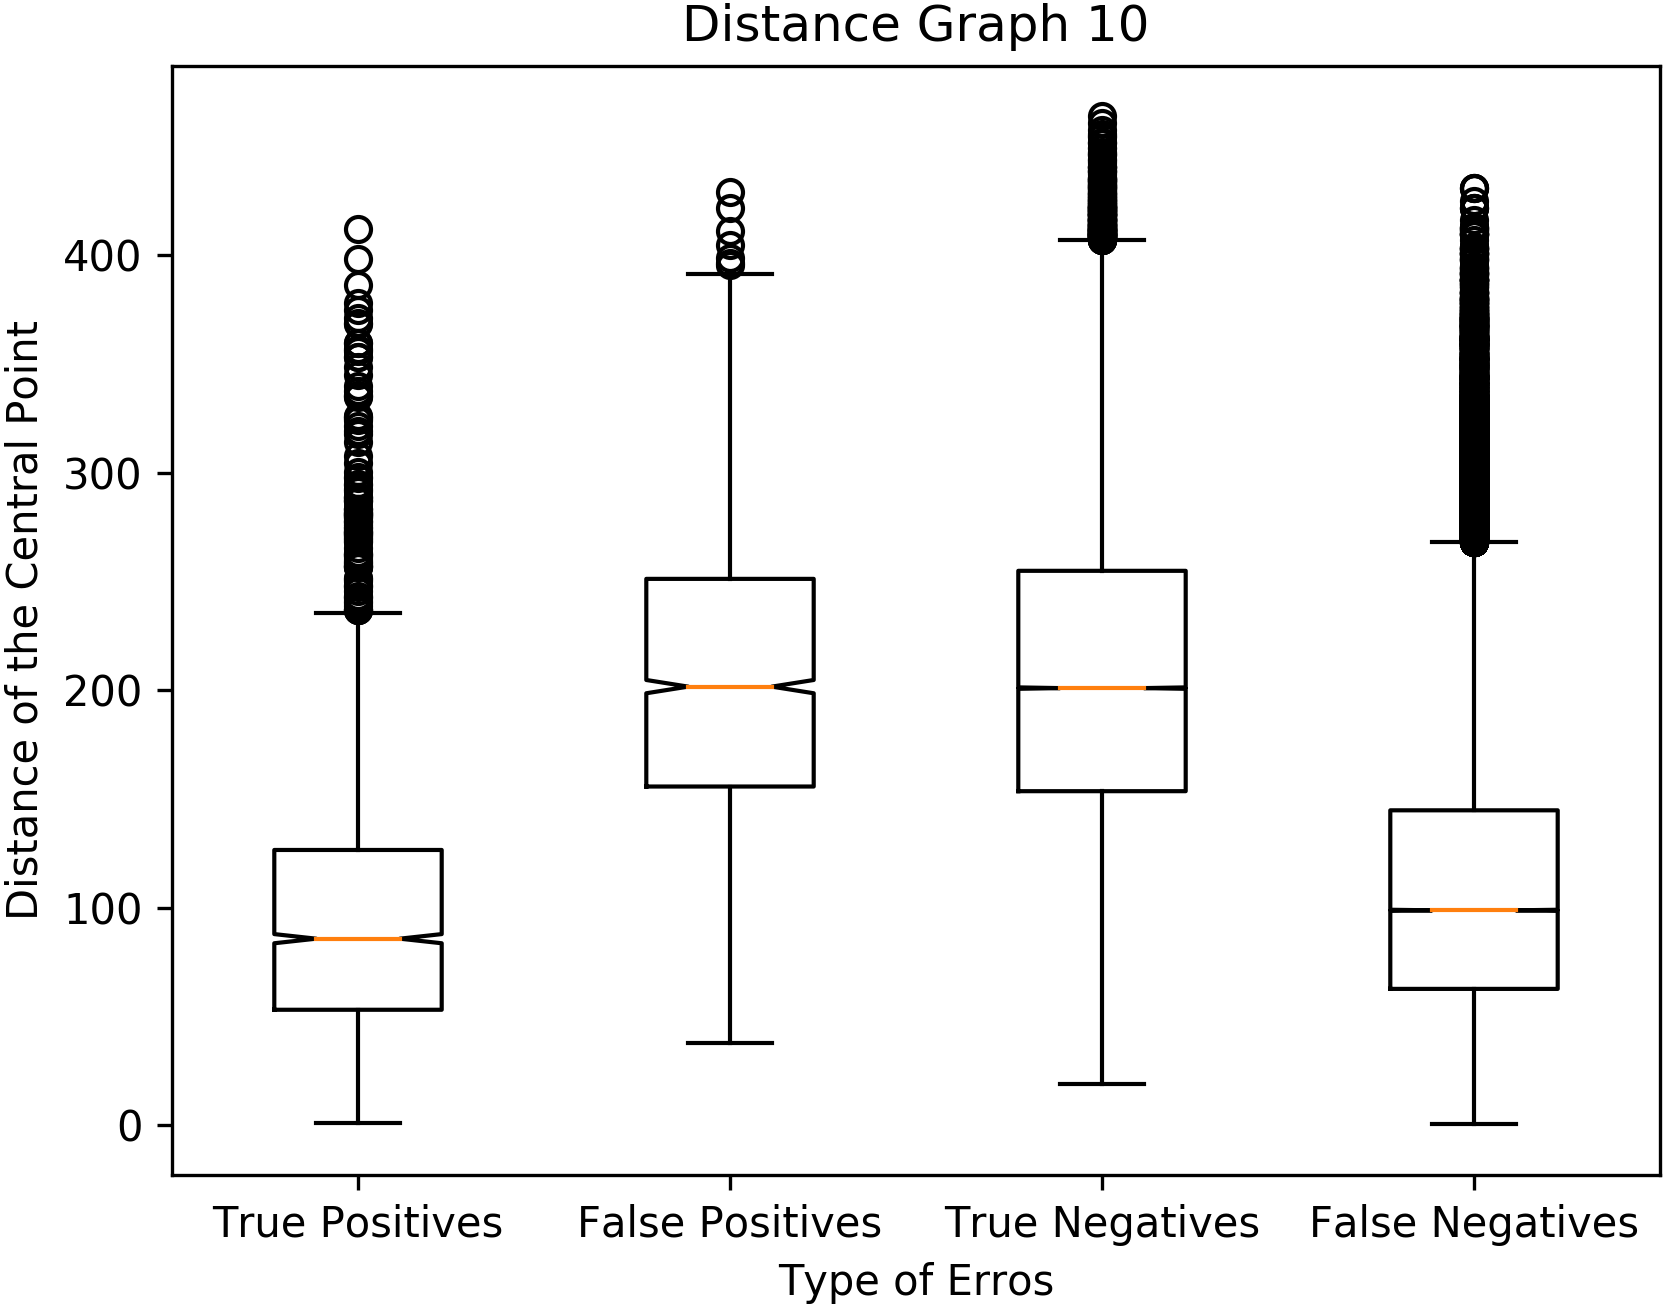
\includegraphics[width=1\linewidth]{img/boxplot-10.png}
		\caption{Exibição das distâncias e valores de erro do \textit{data set} 09 em cada tipo de região.}
		\label{fig:bp-10}
	\end{figure}

	O tempo médio gasto para treino e teste, utilizando os parâmetros e \textit{data sets} mencionados, é de 218,6 minutos com um total de 4131\footnote{Soma de todos os quatro \textit{data sets} e com o de face: $290 + 285 + 274 + 302 + 2980$.} imagens. Com isso, cada é treinado cerca de $ 3,17 $ imagens por segundo. Para validação, o tempo gasto foi de 8,05 minutos avaliando 539\footnote{Dois \textit{data sets} de $259 + 280$.} imagens ao total.

\section{Conclusão} \label{sec:conclusao}
	Por mais que exista ferramentas de fácil acesso e gratuitas, todas elas exigem conhecimento em teoria de inteligência artificial para sua interpretação de arquitetura, funcionamento e suporte e principalmente em sua configuração para a obtenção de resultados mais promissores.
	
	Para o desenvolver deste trabalho, não é necessário ter conhecimento no tema de processamento digital de imagens, entretanto, deve-se ter conhecimento em teoria convolucional de imagens para escolher parâmetros adequados para cada tipo de solução requisitada. Este trabalho baseou-se nos relatos de Garcia \cite{Garcia2004} no qual utiliza imagens e máscaras de pequeno porte e obtendo resultados mais promissores do que a utilização de uma rede neural totalmente conectada, isso sem levar em consideração o gasto energético desta.
	
	Todos os parâmetros utilizados para configuração da rede que não foram explicitados por Garcia \cite{Garcia2004}, como \textit{rate learning} e \textit{momentum} foram obtidos de forma empírica, avaliando o resultado obtido, alterando os valores e realizando novos testes.

	\subsection{Trabalhos Futuros}
		Uma possível forma para melhorar os resultados seria modificar o \textit{data set} de faces de forma a rotacionar e redimensionar as tais para que se tenha mais situações mapeadas em treino, reconhecendo mais faces que não estão posicionadas em perfil ou com com leves giros. Também realizar um filtro nas imagens do \textit{data set FDDB} para utilizar as faces que estão visíveis e sem obstrução para treino a fim de deixar a rede mais abrangente para outros tipos de disposição de faces.
		
		Alterar o parâmetro de aprendizagem do algoritmo para que consiga diferenciar por sí só com mais certeza as regiões apresentadas à ele.
		
		Alteração do processo de criação de saída selecionando o contorno de maior área que abrange o maior espaço que contenha a face, eliminando todos os seus sub-quadrados internos.
		
		Outra possível modificação no trabalho seria alterar as saídas da rede neural. Atualmente, possui-se duas saídas dizendo a probabilidade de cada uma. Poderia realizar uma modificação de forma a colocar somente uma saída, mostrando a porcentagem de ser ou não uma face.

%==========================================
\iffinal

\fi
%==========================================

% trigger a \newpage just before the given reference
% number - used to balance the columns on the last page
% adjust value as needed - may need to be readjusted if
% the document is modified later
%\IEEEtriggeratref{8}
% The "triggered" command can be changed if desired:
%\IEEEtriggercmd{\enlargethispage{-5in}}

\bibliographystyle{IEEEtran}
\bibliography{bib_extra/IEEEabrv,example}

\section*{Anexos}
	\begin{figure}[ht]
		\centering
		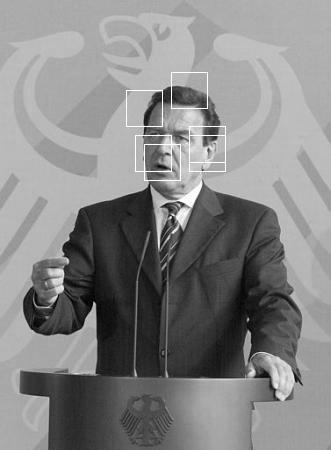
\includegraphics[width=0.65\linewidth]{img/detect_2.jpg}
		\caption{Resultado do processamento de reconhecimento de face no qual retornou com sucesso a face detectada.}
		\label{fig:detect_2}
	\end{figure}

	\begin{figure}[ht]
		\centering
		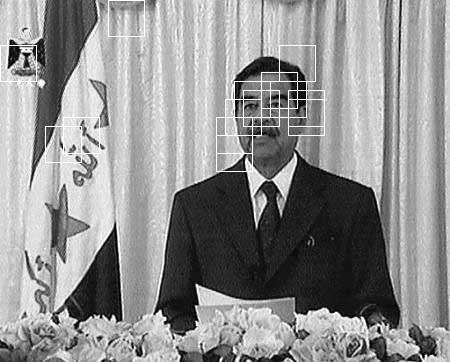
\includegraphics[width=0.75\linewidth]{img/detect_3.jpg}
		\caption{Exemplo de processamento de reconhecimento de face no qual não obteve sucesso total na detecção de todas as faces. Resultado com Falso Positivos, no emblema, na bandeira e na cortina.}
		\label{fig:detect_3}
	\end{figure}

	\begin{figure}[ht]
		\centering
		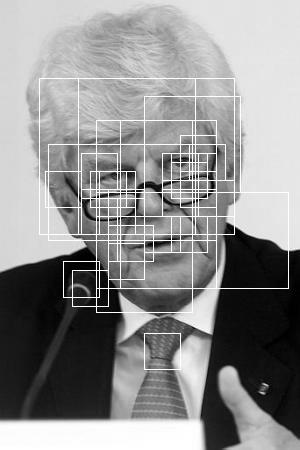
\includegraphics[width=0.7\linewidth]{img/detect_4.jpg}
		\caption{Exemplo de processamento de reconhecimento de face no qual não obteve sucesso total na detecção de todas as faces. Resultado com Falso Positivos, na gravata, no terno e no microfone.}
		\label{fig:detect_4}
	\end{figure}

	\begin{figure}[ht]
		\centering
		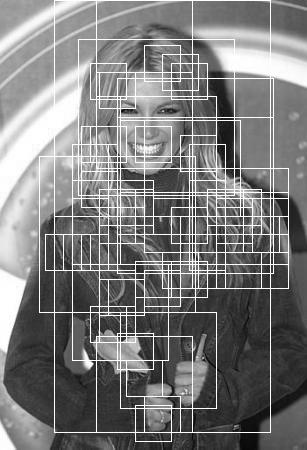
\includegraphics[width=0.75\linewidth]{img/detect_5.jpg}
		\caption{Exemplo de processamento de reconhecimento de face no qual não obteve sucesso total na detecção de todas as faces.}
		\label{fig:detect_5}
	\end{figure}

\end{document}

%==========================================
